\section{Using ``Anim By Sound'' with multiple
tracks}\label{using-anim-by-sound-with-multiple-tracks}

Note. The following "walk through" tutorial is for using Anim By Sound
with multiple tracks. This tutorial is based on my initial experiments
with Anim by Sound and may be revised as I gain more experience. The
tutorial demonstrates using sound to animate a fractal offset parameter
and the material color. The settings file also includes animation of
some other parameters, and produces an animation just over a minute
long, at 300 x 300, 45 minutes to render.

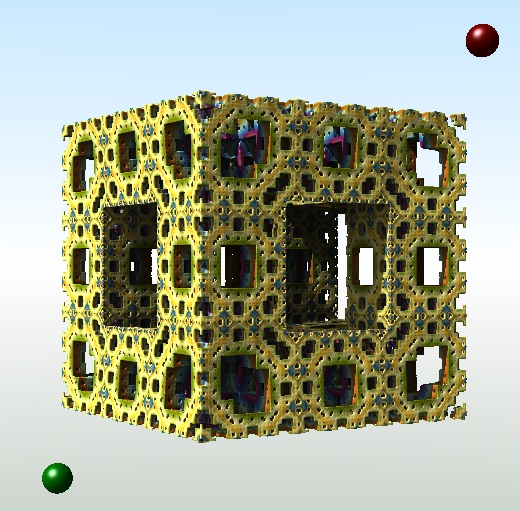
\includegraphics[width=2.63000in,height=2.58000in]{img/sound/media/image1.png}

Animations can take many hours to render, so it is best when learning
the controls, to keep it simple. Choose fractals and/or primitives that
render fast. Do not use slow effects like Volumetric Light of Multi Ray
Ambient Occlusion. I drop the resolution to 400 x 300 Detail Level 0.5,
or 200 x 150 Detail Level 0.25.

The animation value of an object (or an effect) at each frame, is the
sum of the parameter value, (generated from the keyframe animation
table), and the sound value at that frame.\\
animVal = paraVal + soundVal.

This tutorial is about the basics of using soundVal to vary animVal. So
I will keep paraVal constant and use only sound data to direct the
animation of parameters.

A cool thing about using only soundVal (no keyframe animation) is that
we can set up a trial with just two keyframes (beginning and end).

\emph{Note. You can create an audio file for the single purpose of
directing animation, where the audio file is not used at all in the
final song mix. You can use Anim by Sound to create silent videos.}

\emph{Keyframe animation requires changes to be made at keyframes. It is
possible with Sound animation to make changes at any frame, (i.e. a
change at any 1 / 30 of a second time interval, when at 30fps.)}

\emph{Previously, choreographing parameters with spreadsheets was very
time consuming and I was limited to what I could achieve, so I stopped
and have waited. Anim by Sound has made this process much more simpler,
and has infinite possibilities.}

All files used in this example can be downloaded from mandelbulber.org

http://cdn.mandelbulber.org/doc/audio/9\%20tut.zip

unzip and place ``9 tut'' folder in home/mandelbulber/animations/

\subsection{Audio Files}\label{audio-files}

The following formats are supported:

- *.wav (wave form audio format)

- *.ogg (Ogg Vorbis)

- *.flac (Free Lossless Audio Format)

- *.mp3 (MPEG II Audio Layer 3) - supported only under Linux

I used Hydrogen Drum Kit emulator to make all the individual drum track
files. These are .wav files but as I am using Linux I converted them to
.mp3 to use in Mandelbulber. These are mono working files, when I make
the video in VirtualDub I then use the final song mix .wav file.

The guitar tracks have also been recorded as .wav, and a .mp3 copy made
to use with Mandelbulber.

The audio file data is sampled at every frame point, the data is then
converted to a \emph{sound} number ranging between 0 (silent) and 1
(maximum) which can represent Amplitude or Pitch. This value is shown in
the Sound Animation chart on the Audio Selector UI. We can use either
the default Amplitude mode or choose Sound Pitch mode to animate.

For this example I used Pitch with lead guitar (melody line) creating
the fractal movement, and Amplitude for a drum to alternate the color.
The fractal shape will respond to the free flowing melody line and the
color change as a repetitive rhythm event.

This is a screen-shot from Audacity showing some of the instrument
tracks I had available. I only used one drum (a kick drum), but normally
I would be using more percussion instruments.

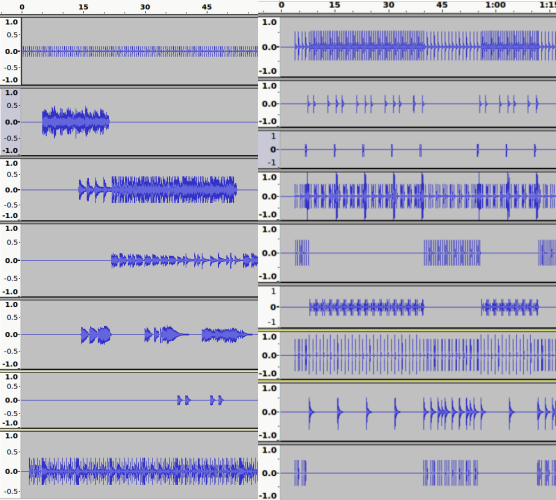
\includegraphics[width=5.04000in,height=4.53000in]{img/sound/media/image2.png}

\subsection{Adding a parameter.}\label{adding-a-parameter.}

Firstly, have the Animation Dock open. ( i.e. from menu select View -
show animation dock.)

Then go to the dock or tab for the parameter you wish to animate (e.g.
fractal, material, effect etc). Right mouse click on the parameter
field, and select Add to Keyframe Animation.

The parameter will then be listed in the keyframe animation table, with
Anim By Sound in the next column.

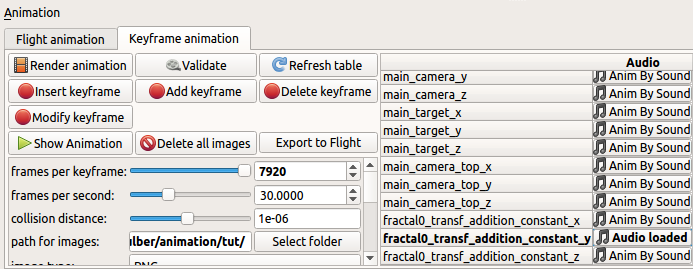
\includegraphics[width=6.69000in,height=2.60000in]{img/sound/media/image3.png}

Here I have chosen to animate parameter Menger\_Mod1 offset y

fractal0\_transf\_addition\_constant\_y

i.e parameter name \emph{transf\_addition\_constant\_y;} from formula
slot \emph{fractal0.}

Parameters x \& z are also added because this parameter is part of a
vector3.

\subsection{Loading the Audio File}\label{loading-the-audio-file}

Left mouse click on Anim By Sound and the Audio Selector UI will open.
The name of the parameter will be in the description along the top.

Select an Audio file and three charts will appear.\\
Enable Animation by Sound and the options will appear.

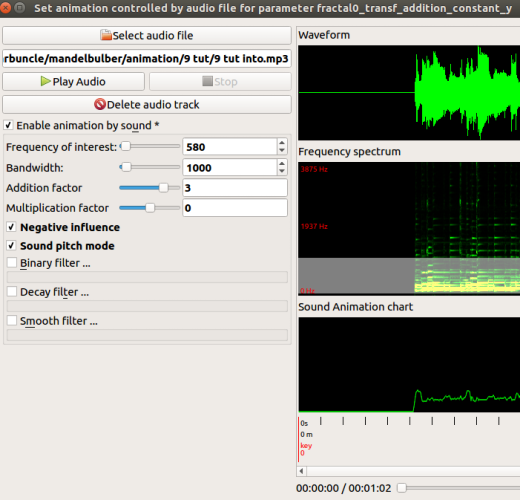
\includegraphics[width=5.42000in,height=5.21000in]{img/sound/media/image4.png}

Animation of a parameter is created by applying an addition-factor
and/or a multiplication-factor.

animVal = paraVal + soundVal.

soundVal = (paraVal * multiplication-factor * \emph{sound)} + (
addition-factor * \emph{sound})

It is less complicated when learning, to use only the addition factor,
so we change multiplication factor to 0.0.

\subsection{Using Sound Pitch mode.}\label{using-sound-pitch-mode.}

I set frequency at 580Hz and bandwidth to 1000Hz, this covers the range
of the fundamental frequencies of my lead guitar notes ( I am removing
higher harmonic frequencies, although this may not be necessary).

Make further adjustment if the Sound Animation charts shows that the
pitch is contained only in the top or bottom of the chart, (resulting
from a melody line only using high notes or only using low notes.) Push
the Play Sound button and check that the chart line is following the
pitch of the audio track.\\
The main point is not to limit the Pitch by having a small band width
that does not cover the full spectrum of the fundamental notes used in
the audio track.

In Pitch mode the Sound Animation chart rises from silent to high pitch.

In this image the \emph{sound} varies from about 0.2 up to almost 1.0
(maximum \emph{sound}). Therefore the \emph{sound} will have a wide
effect on the parameter animation.

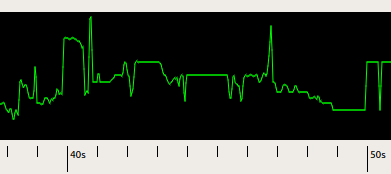
\includegraphics[width=4.07283in,height=1.81260in]{img/sound/media/image5.png}

In this image the \emph{sound} is fairly constant at around 0.2, so it
will have a narrow effect on the animation.

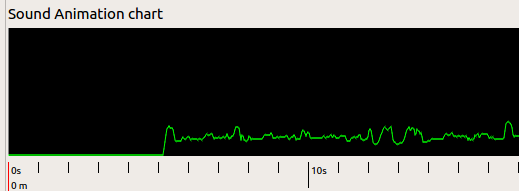
\includegraphics[width=5.40630in,height=1.98976in]{img/sound/media/image6.png}

\subsection{Testing the parameter}\label{testing-the-parameter}

Close the Audio Selection UI and go the Menger\_Mod1 fractal tab and
test the parameter through a range of values.

\emph{If a parameter belongs to a fractal formula, you may notice that
the ray marching step multiplier needs to be adjusted to produce a good
image throughout the animation range.}

\emph{As a guide for adjusting the ray marching step multiplier, open
View - Show statistics, and monitor Percentage of wrong distance
estimations.}

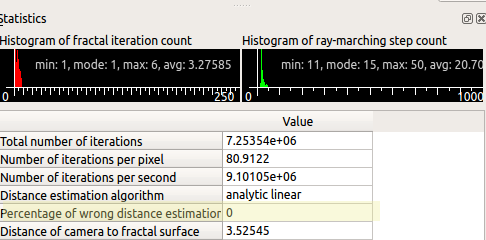
\includegraphics[width=5.40827in,height=2.67087in]{img/sound/media/image7.png}

Now I decide on the appropriate size of the addition factor to use for
animating the parameter.

I have paraVal ``offset y'' set at a constant value of 0.0, and I test
an addition factor of 3.0. The \emph{sound} will increase the soundVal
in the range of 0.0 to 3.0 maximum. However for the effect I want, I am
be using Negative influence mode, which will subtract the soundVal from
paraVal instead of adding it, therefore the possible range to be tested
is 0.0 to -3.0.

The audio file I used only creates \emph{sound} between 0.0 and about
0.2, so the offset values I will be testing are the actual range between
0 and -0.6, i.e. 0.0 = 0.0 * -3.0 max, -0.6 = 0.2 * -3.0 max.

\emph{Note: There are two types of parameters in this program. The first
type can have negative values entered, the second type cannot. It is}
\emph{important} \emph{when animating a parameter of the second type,
that the functions and settings used, do not result in a negative
number.}

View the Sound Animation chart to see the what values you are likely to
get from \emph{sound} at different parts of the instruments music.

Remember to set the parameter back to the original value when you have
finished testing.

\subsection{Using Amplitude}\label{using-amplitude}

Example: Animate the color of the fractal on every beat of the kick
drum.

Add material 1 parameter ``Palette\_offset'' to the Keyframe animation
table.

Open Anim By Sound, load audio file and Enable Animation by sound.

Adjust Frequency of interest and bandwidth.

Enable ``Binary filter'' and adjust the threshold so that all the beats
are shown in the Sound Animation chart.

Here I am creating an event (at every kick drum beat), that lasts for a
minimum duration of 7 extra frames (7/30 seconds). The event is using
Addition factor * sound and is triggered every time the sound amplitude
increases above the threshold (0.400) and will last for 7/30 seconds.
Events that last less than ``say'' 7 frames are difficult to observe at
30 fps.

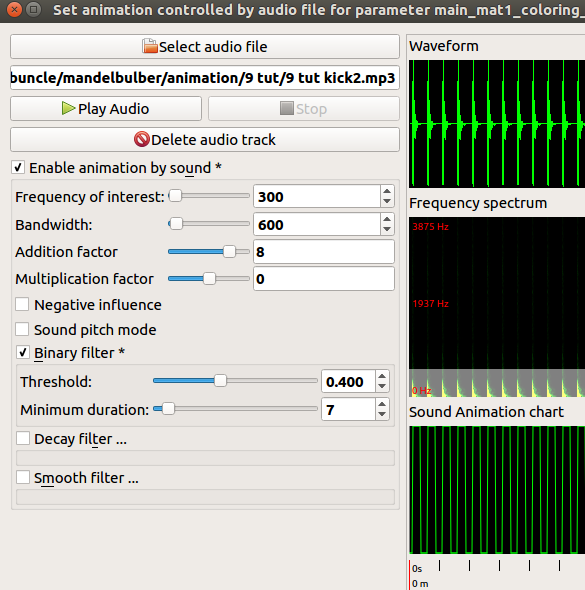
\includegraphics[width=5.24528in,height=5.29016in]{img/sound/media/image8.png}

\subsection{Rendering the animation.}\label{rendering-the-animation.}

First add two identical keyframes to the Keyframe Animation table,

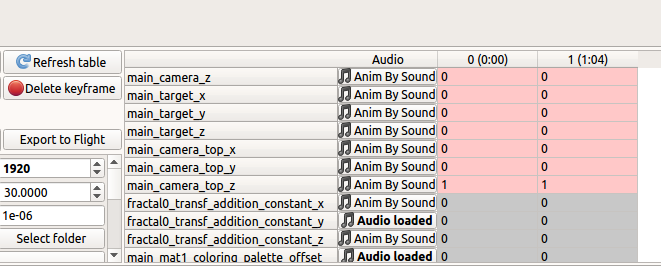
\includegraphics[width=6.69291in,height=2.69291in]{img/sound/media/image9.png}

and set ``frames per keyframe'' to a number that will cover the length
of the trial, i.e. for 64 seconds at 30 fps it would be:

64sec * 30fps = 1920 frames per keyframe.

Make sure that the ``path for images'' is linked to the correct folder,
and ensure that the folder is empty, ``Delete all images'' button.

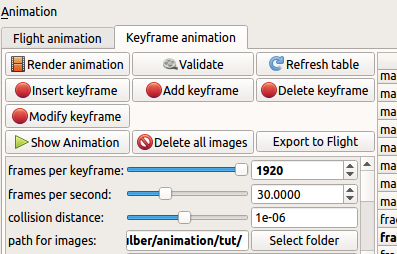
\includegraphics[width=4.14000in,height=2.65000in]{img/sound/media/image10.png}

\subsection{Now render the trial
animation.}\label{now-render-the-trial-animation.}

When rendering is finished (note the time it took) , press ``Show
animation'' button for a preview (you can also use ``Show animation''
while rendering is in progress.)

I also create a video with VirtualDub and the audio file, to ensure that
the animation is working correctly with the sound. If the animation is
satisfactory, then set the resolution and detail level to your final
settings and wait.
